\documentclass[a4paper,11pt]{article}
\usepackage[T1]{fontenc}
\usepackage[latin1]{inputenc}
%\usepackage[polutonikogreek]{babel}
\usepackage{amssymb} %math-befehle
\usepackage{fancyhdr} %kopf- und fusszeile
\usepackage{a4wide}
\usepackage[top=20mm,left=20mm,right=20mm]{geometry} %seitenraender
%\usepackage[paper=a4paper,left=25mm,right=25mm,top=20mm,bottom=25mm]{geometry} %seitenraender
\usepackage{parskip} %kein einzug bei absatz
\usepackage[pdftex]{graphicx} %fuer grafiken einfuegen
\usepackage{color}
\definecolor{LK}{rgb}{0.05,0.05,0.3} %dunkelblau
\usepackage[pdftex,bookmarks=true,bookmarksnumbered=true,colorlinks=true,linkcolor=blue,filecolor=red,citecolor=LK,pdfstartview=FitH]{hyperref} %kapiteldarstellung im pdf file
\renewcommand{\textfraction}{0.15} %lockerere bildpositionierungsregeln
\renewcommand{\topfraction}{0.85}
\renewcommand{\bottomfraction}{0.65}
\renewcommand{\floatpagefraction}{0.60}
\renewcommand{\figurename}{Fig.} 
\newcommand{\Matrix}[2]{\left(\begin{array}{#1}#2\end{array}\right)}
\setcounter{topnumber}{3}
% \addto\captionsngerman{%
 %   \renewcommand{\figurename}{Fig.}%
   % \renewcommand{\tablename}{Tab.}%
  %}
\usepackage[]{natbib} %citep, citet
\newcommand\aj{\ref@jnl{AJ}}%
          % Astronomical Journal
\newcommand\actaa{\ref@jnl{Acta Astron.}}%
  % Acta Astronomica
\newcommand\araa{\ref@jnl{ARA\&A}}%
          % Annual Review of Astron and Astrophys
\newcommand\apj{\ref@jnl{ApJ}}%
          % Astrophysical Journal
\newcommand\apjl{\ref@jnl{ApJ}}%
          % Astrophysical Journal, Letters
\newcommand\apjs{\ref@jnl{ApJS}}%
          % Astrophysical Journal, Supplement
\newcommand\ao{\ref@jnl{Appl.~Opt.}}%
          % Applied Optics
\newcommand\apss{\ref@jnl{Ap\&SS}}%
          % Astrophysics and Space Science
\newcommand\aap{\ref@jnl{A\&A}}%
          % Astronomy and Astrophysics
\newcommand\aapr{\ref@jnl{A\&A~Rev.}}%
          % Astronomy and Astrophysics Reviews
\newcommand\aaps{\ref@jnl{A\&AS}}%
          % Astronomy and Astrophysics, Supplement
\newcommand\azh{\ref@jnl{AZh}}%
          % Astronomicheskii Zhurnal
\newcommand\baas{\ref@jnl{BAAS}}%
          % Bulletin of the AAS
\newcommand\caa{\ref@jnl{Chinese Astron. Astrophys.}}%
  % Chinese Astronomy and Astrophysics
\newcommand\cjaa{\ref@jnl{Chinese J. Astron. Astrophys.}}%
  % Chinese Journal of Astronomy and Astrophysics
\newcommand\icarus{\ref@jnl{Icarus}}%
  % Icarus
\newcommand\jcap{\ref@jnl{J. Cosmology Astropart. Phys.}}%
  % Journal of Cosmology and Astroparticle Physics
\newcommand\jrasc{\ref@jnl{JRASC}}%
          % Journal of the RAS of Canada
\newcommand\memras{\ref@jnl{MmRAS}}%
          % Memoirs of the RAS
\newcommand\mnras{\ref@jnl{MNRAS}}%
          % Monthly Notices of the RAS
\newcommand\na{\ref@jnl{New A}}%
  % New Astronomy
\newcommand\nar{\ref@jnl{New A Rev.}}%
  % New Astronomy Review
\newcommand\pra{\ref@jnl{Phys.~Rev.~A}}%
          % Physical Review A: General Physics
\newcommand\prb{\ref@jnl{Phys.~Rev.~B}}%
          % Physical Review B: Solid State
\newcommand\prc{\ref@jnl{Phys.~Rev.~C}}%
          % Physical Review C
\newcommand\prd{\ref@jnl{Phys.~Rev.~D}}%
          % Physical Review D
\newcommand\pre{\ref@jnl{Phys.~Rev.~E}}%
          % Physical Review E
\newcommand\prl{\ref@jnl{Phys.~Rev.~Lett.}}%
          % Physical Review Letters
\newcommand\pasa{\ref@jnl{PASA}}%
  % Publications of the Astron. Soc. of Australia
\newcommand\pasp{\ref@jnl{PASP}}%
          % Publications of the ASP
\newcommand\pasj{\ref@jnl{PASJ}}%
          % Publications of the ASJ
\newcommand\qjras{\ref@jnl{QJRAS}}%
          % Quarterly Journal of the RAS
\newcommand\rmxaa{\ref@jnl{Rev. Mexicana Astron. Astrofis.}}%
  % Revista Mexicana de Astronomia y Astrofisica
\newcommand\skytel{\ref@jnl{S\&T}}%
          % Sky and Telescope
\newcommand\solphys{\ref@jnl{Sol.~Phys.}}%
          % Solar Physics
\newcommand\sovast{\ref@jnl{Soviet~Ast.}}%
          % Soviet Astronomy
\newcommand\ssr{\ref@jnl{Space~Sci.~Rev.}}%
          % Space Science Reviews
\newcommand\zap{\ref@jnl{ZAp}}%
          % Zeitschrift fuer Astrophysik
\newcommand\nat{\ref@jnl{Nature}}%
          % Nature
\newcommand\iaucirc{\ref@jnl{IAU~Circ.}}%
          % IAU Cirulars
\newcommand\aplett{\ref@jnl{Astrophys.~Lett.}}%
          % Astrophysics Letters and Communications
\newcommand\apspr{\ref@jnl{Astrophys.~Space~Phys.~Res.}}%
          % Astrophysics Space Physics Research
\newcommand\bain{\ref@jnl{Bull.~Astron.~Inst.~Netherlands}}%
          % Bulletin Astronomical Institute of the Netherlands
\newcommand\fcp{\ref@jnl{Fund.~Cosmic~Phys.}}%
          % Fundamental Cosmic Physics
\newcommand\gca{\ref@jnl{Geochim.~Cosmochim.~Acta}}%
          % Geochimica Cosmochimica Acta
\newcommand\grl{\ref@jnl{Geophys.~Res.~Lett.}}%
          % Geophysics Research Letters
\newcommand\jcp{\ref@jnl{J.~Chem.~Phys.}}%
          % Journal of Chemical Physics
\newcommand\jgr{\ref@jnl{J.~Geophys.~Res.}}%
          % Journal of Geophysical Research
\newcommand\jqsrt{\ref@jnl{J.~Quant.~Spec.~Radiat.~Transf.}}%
          % Journal of Quantitiative Spectroscopy and Radiative Trasfer
\newcommand\memsai{\ref@jnl{Mem.~Soc.~Astron.~Italiana}}%
          % Mem. Societa Astronomica Italiana
\newcommand\nphysa{\ref@jnl{Nucl.~Phys.~A}}%
          % Nuclear Physics A
\newcommand\physrep{\ref@jnl{Phys.~Rep.}}%
          % Physics Reports
\newcommand\physscr{\ref@jnl{Phys.~Scr}}%
          % Physica Scripta
\newcommand\planss{\ref@jnl{Planet.~Space~Sci.}}%
          % Planetary Space Science
\newcommand\procspie{\ref@jnl{Proc.~SPIE}}%
          % Proceedings of the SPIE
\let\astap=\aap
\let\apjlett=\apjl
\let\apjsupp=\apjs
\let\applopt=\ao
\newcommand\phn{\phantom{0}}%
\newcommand\phd{\phantom{.}}%
\newcommand\phs{\phantom{$-$}}%
\newcommand\phm[1]{\phantom{#1}}%
\let\la=\lesssim            % For Springer A&A compliance...
\let\ga=\gtrsim
\newcommand\sq{\mbox{\rlap{$\sqcap$}$\sqcup$}}%
\newcommand\arcdeg{\mbox{$^\circ$}}%
\newcommand\arcmin{\mbox{$^\prime$}}%
\newcommand\arcsec{\mbox{$^{\prime\prime}$}}%
\newcommand\fd{\mbox{$.\!\!^{\mathrm d}$}}%
\newcommand\fh{\mbox{$.\!\!^{\mathrm h}$}}%
\newcommand\fm{\mbox{$.\!\!^{\mathrm m}$}}%
\newcommand\fs{\mbox{$.\!\!^{\mathrm s}$}}%
\newcommand\fdg{\mbox{$.\!\!^\circ$}}%

\begin{document}
%%%%%%%%%%%%%%%%%% title page %%%%%%%%%%%%%%%%%%%%%
\pdfbookmark[1]{title page}{tit}

\title{IBIS data reduction, v170413}

\author{Lucia Kleint \\
e-mail: \mbox{kleintl@ucar.edu}
}

\date{August 9, 2017}

\maketitle
\newpage
%%%%%%%%%%%%%%%%%%%%%%%%%%%%%%%%%%%%%%%%%%%%%%%%%%%%

\tableofcontents
\newpage

%%%%%%%%%%%%%%%%%%%%%%%%%%%%%%%%%%%%%%%%%%

\section{Introduction}
\subsection{General}
The IBIS data reduction can be done (more or less) automatically using \texttt{ibis\_gui\_new.pro}. Start with:

IDL> ibis\_gui\_new

The required libraries (see requirements) must be in your !Path variable. The first button of the GUI needs to be pressed each time the GUI (or IDL session) is started to initialize all variables. Some variables, such as paths and wavelengths, may need to be changed for each reduction, which is done in the menu of the first button or directly on the GUI for the observing mode. The first button creates the file ibis\_variables.txt, which saves the current state and restores it in future uses. \texttt{Textbox\_lk.pro} contains the variables of the pop-up window.

The other buttons/programs should be run in their order but one may stop
in the middle and continue on the next day as long as the first button
is always used when restarting the reduction.

The wavelength to reduce is defined when clicking on 'variables'. 
Some parameters (for example kernel size and type of destretch) will
be the same for all wavelengths during one run of the GUI, i.e. if
you define lambda=[8542 6302]. If you want different parameters for
each wavelength, define lambda=[8542] first, run the full reduction,
define lambda=[6302] and re-run the reduction with the different
settings. One also needs to pay attention if for example the exposure
time changed during the day (only one dark will be created, so rerun
the reduction for other dark and corresponding observations).

The kernel size for the destretch is written in kerneltxt.txt. The program checks if
the file exists. If yes, the values in txt file are used, if not, it defaults to [0,64,32,16].

Generally, if there is an overwrite option this means that the first
run of the subprograms will create all necessary files (even for $\lambda$
that were not specified in the beginning). Re-running and setting the
overwrite option should not be necessary in general.

If the polcal was taken on a different date, specify its path in first
textbox (all subdirectories will be searched). Format should be
similar to 'path to original data', which will be chosen in case
polpath is not defined in the textbox.

Starting with v4, a complete .tex log of all data reduction steps and
important images is created in a subdirectory called \textit{log}. You
need to manually compile it \textit{latex log\_datared.tex} (often more than
once to get the labels right), then \textit{dvips log\_datared.dvi}
and \textit{ps2pdf log\_datared.ps}. Sometimes the \textit{clearpage}
command will need to be inserted if the compilation is not working. This may happen when many images were inserted with little text (for example when one reduces a dozen timestamps).

This version of the GUI no longer supports pre 2010 data (that were
taken with a different camera and a different file system). v5 of the
GUI works fine for those. The main change from v5 to this version (newred) is
the alignment: now all data in all wavelengths should be aligned in
the end. Currently, IBIS creates one fits file per scan and all
images, filters, polarization states are in extensions. Also new is
the possibility to run the polcal with fewer than 4 table positions. I
verified that even just one table position gives the same X matrix
(using 2 positions is still recommended).

Many subprograms were taken from A.~Tritschler's version of the data reduction but there are significant differences in programming, user handling and variable names, so that the two versions are not compatible. Major differences between the two versions include a totally rewritten polcal by T. Schad (with the same X matrices as result) and minor differences in beam combination, size of speckle files, the alignment procedure and various bug fixes. Also, the prefilter is now applied to the gain (as of June 2015) and thus all data are corrected for the prefilter transmission automatically.

\subsection{Requirements}

All necessary routines should already be included in the ibis\_newred directory and its subdirectories. All you need to do is to also include the subdirectories in the IDL path. Earlier versions required to adapt ftsread.pro for the absolute path to fts\_cent.dat, but newer versions (as of July 2017) should not require this.

textbox\_lk.pro (which opens a widget in this widget to manually
         select paths etc.) \\
          coyote library (fanning) \\
          mpfitellipse (directory called 'fitting') \\
          buttonbox\_lk.pro\\
          xline, yline, diffelement, xy, anim\_lk (for other routines)\\
          astrolib (for find\_all\_dir etc.) 
                       (downloaded from: http://idlastro.gsfc.nasa.gov/ftp/) \\
          where2d (ssw) 2-dimensional where\\
          several routines from solarsoft (directory called fromssw) \\
          ftsread.pro 

\newpage
\section{General Description of IBIS and the Data Reduction}
Here we describe IBIS and the general steps required to reduce Fabry Perot data\footnote{A significant part of this section is taken from my Diploma thesis (Kleint 2007, ETH)}. The IBIS pipeline follows this scheme.

\subsection{IBIS}
The Interferometric Bidimensional Spectrometer (IBIS) developed by the INAF/Arcetri Astrophysical Observatory was installed at the Dunn Solar Telescope in 2003. In November 2006 an extension was installed which allows to perform polarimetric measurements. It consists of two liquid crystal variable retarders (LCVR) and a polarizing beam splitter (PBS), drawn in color in Fig.\ref{img:ibis}. The primary light path is shown by the solid line.\par
\vspace{-2pt}
\begin{figure}[h!]
\begin{minipage}[t]{0.55\textwidth}
\vspace{0pt}
\centering
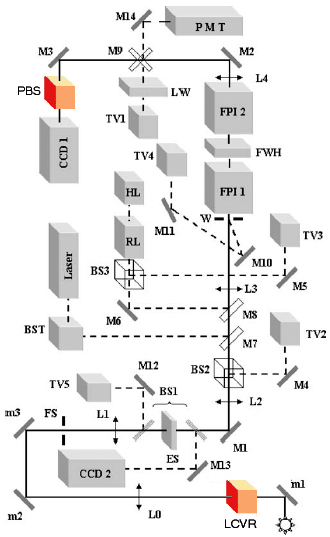
\includegraphics[width=\textwidth]{ibis.jpg}
	 \vspace{-26pt}\caption{IBIS setup (adapted from \citet{cavallini2006})}\label{img:ibis}
\end{minipage}
\hfill
\begin{minipage}[t]{0.45\textwidth}
\vspace{3pt}\sffamily
 Abbreviations used for IBIS:\\
 \begin{tabular}{p{0.8cm} l}
 &\\
 BS: & beam splitter\\
 L: & lenses\\
 M,m: & mirrors\\
 & \\
 CCD: & camera\\
 TV: & camera\\
 & \\
 LCVR: & liquid crystal variable retarder\\
 PBS: & polarizing beam splitter\\
 & \\
 FPI: & Fabry Perot interferometer\\
 FWH: & filter wheel\\
 &\\
 BST: & beam steering\\
 ES: & common mechanical shutter\\
 FS: & field stop\\
 HL: & halogen lamp\\
 LW: & lens wheel\\
 PMT: & photomultiplier\\
 RL: & relay lenses \\
 W: & window\\
 \end{tabular}
\end{minipage}
\end{figure}
\vspace{-5pt}
m1 is located just after the exit of the adaptive optics system (tip tilt + 97 actuator deformable mirrors). On the primary beam the light passes through two LCVRs (inside one box) which modulate its polarization state. The exchangeable field stop (FS) determines the size of the image on the chip. Due to the electronic shutter, the narrow band IBIS image on CCD 1 and a white light image on CCD 2 are taken simultaneously. The prefilter (FWH) restricts the spectral region that is observed. With the voltage-tunable Fabry-Perot interferometers scanning through the selected line profile can be performed. The light then goes through the PBS which consists of a modified Savart plate and which splits the incoming beam into two orthogonal polarization states. On the CCD 1 chip two images of orthogonal polarization states are taken at the same time resulting in the advantage of same seeing for both.

The reference path is illustrated by the two dashed lines originating in BS1. The path before the ES ends in TV5, a camera that shows the selected solar region live. Its use is to watch the seeing and to see if the position on the Sun is kept. The second path ends in CCD 2, which is the white light (broad band) camera. It is used as a reference to the narrow band images to determine positional shifts and seeing. For example, the light level drops if clouds are present, which sometimes cannot be seen in the narrow band images but is clearly visible in white light.

\subsubsection{Collimated vs. Telecentric Mount}
There are two possible mounts for the FPI's: collimated (classic) or telecentric mount. In classic mount the FPI's are mounted near an image of the entrance pupil of the telescope (=pupil plane). The image is formed through rays incident on the FPI's with different angles. This gives a systematic wavelength shift across the field of view, which has to be determined and corrected during data reduction. With respect to the center of the field of view, the passbands in all other regions get blueshifted. In telecentric mounts, the pupil image is collimated and the FPI's are placed near an image plane of the Sun. All rays that originate in the same field point pass the FPI's with different angles but in the same point. This leads to a broadening of the transmission profile but not to a wavelength shift across the field of view. For maximum spectral resolution the opening angle of the beam has to be minimized. Examples for collimated mounts: IBIS (NSO), IRSOL-FP. Examples for telecentric mounts: TESOS (VTT), VIS (BBSO).

Possible problems of the telecentric mount are dust particles which have a higher influence than in classic mount. This can be solved by flat-fielding. Another problem in telecentric mount is fringing which occurs when parallel reflecting surfaces are present in an image plane. Fringing can also be removed by flat-fielding but only if the fringes are constant during the observing run which requires a constant temperature \cite{cavallini2006}. An advantage of classic mount is that the transmission profile has the same shape for all points of the beam since the FPI's and prefilters are near the pupil plane. Near an image plane as in the telecentric mount, the transmission profile does not have the same shape in every point even though this can be mediated by having a large F-number. Considering all this reasons, a classic mount has been chosen for IBIS.

For IBIS, the FPI's are operated in axial-mode. This means, the optical axis is perpendicular to the plates of the Fabry-Perots. In most cases this is not desirable because a collimated beam on a FPI produces a reflected and a transmitted beam. These reflections between the FPI's produce ghost images at the final focal plane. Therefore, the plates of the FPI's are often tilted or wedged. Since there are disadvantages from tilting, such as inhomogeneous darkening of the field of view and less transmittance, another solution has been adopted in IBIS. The prefilters are situated between both interferometer plates and block most of the reflections. In this way no tilting is necessary which gives maximum possible transparency and the ghost images are reduced.

IBIS uses two FPI's. A consequence of such a free spectral range is that very narrow-band prefilters (FWHM 3 - 5 \AA) have to be used and therefore not every line can be scanned in its whole range.



\subsubsection{Calibrations}
During the observing setup, or sometimes every morning, several calibration steps are performed. 

\textbf{Etalon orientation and parallelism}\\
A pair of beam splitters (BS2) can be inserted in the light path with the goal to adjust the FPI's perpendicular to the beam. Two overlapping images can be seen on TV2. This is done for every FPI separately with the other one removed from the beam. The FPI's can be moved around two axes and therefore adjusted until the images overlap perfectly. Every other path is then aligned with respect to this first path without moving the FPI's anymore. The perpendicularity is critical since the transmission of the FPI's and the passband of the prefilters depends on the incident angle.

The laser path is used to check the parallelism of the plates of the interferometers.  A circular rotating diffuser makes the frequency stabilized He-Ne laser light incoherent. It is useful to have homogeneous, spectrally incoherent light, since coherent laser light would produce constant speckles due to interference effects which could be misinterpreted as defects on the plates. With M7 and M9 inserted the light goes to the lens wheel that has three different lenses and falls on TV1. With one FPI in the beam and the other one removed from the light path parallelism errors can be made visible as brightness inhomogeneities on TV1. The image on TV1 should change uniformly when changing the plate spacing by applying different voltages. Plate defects are visible as dark spots on the image. Experience has shown that the parallelism is constant during the observing run but nevertheless this check is performed each morning.

\textbf{Lamp tuning}\\
The lamp tuning is used to find the alignment and transmission of the FPI's and the prefilters.
The tuning path starts at the halogen lamp (HL). This lamp has a flat spectrum (not overall, but close enough for scanning the spectral lines) which is necessary for the calibration of the spacing of the FPI's. The RL make the  image to be of the same size as the solar image. M8 and BS3, a pair of beam splitters similar to BS2, is used to check the perpendicularity of the lamp light to the FPI's. Two overlapping images can be seen on TV3. TV4 shows the position of the beam on the diaphragm. The images on TV3 and TV4 have to overlap and be centered by simultaneously moving M6 and M8. If this is done and the M9 mirror is in the right position, the PMT detects an integrated light level. Then the FPI's are calibrated, which means varying the voltage to find the transmission peaks. This has to be done for every filter separately since the transmission profile is wavelength dependent. At first, FP1 scans in big steps and then in smaller steps while FP2 is held at a fixed voltage. The output intensity is recorded with the PMT. Once the maximum transmission is found both transmission profiles coincide. Then both FPIs are moved simultaneously to find the maximum transmission and therefore avoid transmission fluctuations due to small tuning errors. In the fifth step the center of the prefilter profile is found. With that the program can determine the useful range of voltages so that the observations stay in the range of the prefilter. Only the voltages for both FPIs corresponding to the center of the passband are stored.


\textbf{Spectral scans and wavelength definition}
The spectral scans have the aim to determine the voltage to wavelength conversion of the FPIs. The wavelength definition menu then generates an observing file with information about the desired wavelength steps of the observations. Spectral scans are performed with the solar beam and not the halogen lamp. The wavelengths of the solar lines are known (atlas) and by going through the wavelengths of the selected prefilter and recording the intensity it crosscorrelates the observations with the atlas. This gives a voltage to wavelength conversion for the FPIs. The method is not perfect since solar lines can change their position by Doppler shifting, but close enough for the observations. After the spectral scans the user can choose an input file with desired wavelengths and the IBIS program converts these wavelengths to voltages for the FPIs using the scale obtained from the spectral scans.

\subsection{Data Reduction Steps}
The steps described in this section are generally valid for the data reduction of FP data. Abbreviations used are NB for the narrowband (spectral) data and WL for the white-light (broadband) data.

\begin{itemize}
\item Create a dark and a flat for the WL data by averaging the respective observations. The final flat has  the average dark subtracted. At least 200 images are used for each average.
\item Align the NB to the WL through rotation and shifting. Ideally, the WL should be aligned to reference data (e.g. HMI), but this is currently not done for IBIS.
\item Create a dark for the NB data by averaging the respective observations.
\item Create flats for the NB data. This is more complicated than WL because there is an intensity variation in wavelength due to the spectral line and the prefilter transmission. Also, for collimated mounts, there is an intensity variation across the FOV in the shape of concentric rings. Therefore, the steps are as follows: 
\begin{enumerate}
\item Have at least 30 flat images per wavelength and polarization state and average them to get rid of solar intensity variations, then subtract average NB dark. This assumes that the flats were taken with the telescope pointing moving randomly.
\item For collimated mounts: The blueshift of the instrumental profile / redshift of the spectral line across the FOV needs to be calculated. For each pixel in the flat and separately for the L and R beam, first interpolate the wavelength scale (here to equidistant 10 m\AA, quadratic interpolation). Then find the line center of each pixel. For IBIS, this is done with a 3rd deg polynomial and with the center of gravity method. The position of the minimum or the COG then is seen to vary across the FOV in concentric rings. Care needs to be taken to fit only one line (e.g. manual selection in case of 6301/6302). The last step is a quadratic surface fit, giving one POLY\_FIT and one COG fit map of the shift.
\item Construct the gain. For collimated mounts, the influence of the blueshift on the flat needs to be removed, therefore the blueshift needs to be calculated before this step. The wavelength of each pixel in the flats is interpolated onto a common equidistant 10 m\AA\ scale. The center of the FOV (IBIS: 100x100 pixels) is averaged to obtain a typical flat profile. One should not average a too large FOV otherwise the profile is broadened due to the averaging of differently shifted profiles. A map of the typical flat profile is created where the profile is shifted according to the required blue/redshift for each pixel (choose beforehand whether COG or POLY looks better). This creates an average profile map and deviations from this map are considered to be due to dust/imperfections/prefilter. Save the intensity difference between left and right beam (cfactor in code). The final flat without spectral lines is obtained by calculating ``measured flat / (shifted typical profile map)''.
\item For the telecentric gain, one can probably just normalize each flat wavelength to 1 and this will get rid of both the prefilter intensity variation and the spectral line in the gain.
\end{enumerate}

\item Obtain the prefilter profile. This step requires that the general transmission profile is known (e.g. from the manufacturer, or better through own measurements, for example from a scan with the halogen lamp). For IBIS, the profile does not vary significantly across the FOV, apart from fringes, which currently are not taken into account (amplitude variation of 2\% in final data). It can however be shifted in wavelength, depending on the tilt of the prefilter and because for IBIS, the optical path between prefilter measurements (with PMT) and observations (with cameras) is different. The steps are:
\begin{enumerate}
\item Broaden the atlas by the IBIS FWHM and shift the atlas to correct wavelengths (strangely, my copy of the FTS atlas has a 40 m\AA\ shift of the 8542.1 line for example).
\item Cross-correlate the flat to the atlas to find the wavelength-offset of the data, which have the same wavelength scale as flats. IBIS only has relative wavelengths, not absolute wavelengths in the headers.
\item wavelength-shift prefilter profile relative to spectral scan for best match (crosscorrelation) with atlas
\item save the prefilter wavelength scale (new) and the prefilter transmission.
\end{enumerate}

\item Now correct the gain intensities with the prefilter intensities, i.e. gain = gain$_{old}$ / ip\_pref, where ip\_pref is the interpolated prefilter. This step means that the intensities of the final data will be properly corrected, thus preserving the line profiles.

\item Prepare the WL input for the speckle code (save several images in one file in binary format), run the speckle code and reimport the images into IDL. NB data are not speckled because speckle changes the contrast and thus may change the polarization fraction.
\item Destretch the speckle images to have a uniform time series. Best would be to destretch them with reference to HMI (or any seeing-free reference), but this is currently not done.

\item Correct NB data:   data = (data - dark) * gain. Apply the alignment parameters for the L+R beam and for NB to WL alignment, so that one gets the arrays WL=[x,y,time] and NB=[x,y,wavelength,Stokes, beam].
           
 \item This step is optional and depends on your interpretation of seeing. The atmospheric dispersion creates a wavelength-dependent shift and therefore NB and WL are offset (up to 15 px in IBIS!). One can therefore crosscorrelate NB and WL and shift NB onto WL. If the turbulence occurs close to the telescope, then this step may need to be omitted because the turbulence should depend on the pixel location on the camera and not the solar region. In this case, one should do the destretch applying the same vectors to the same pixels in e.g. 8542/6302 (independent of the solar features there) and find the shift due to dispersion between the wavelengths after the destretch. However, because the seeing depends on wavelength anyway, both options may not be great and the shifts may need to be scaled down for longer wavelengths. I have never compared any of these options.
 
 \item Final correction of NB data: WL data are divided by the light level taken from headers. WL data are then destretched with respect to the speckle reconstructed image for that scan and the shifts are saved. The NB data are shifted according to the shifts that were found earlier and same for the blueshift maps. Now the cubes contain the same solar position in each pixel for each wavelength. Only then can the line profiles be interpolated and shifted to a common wavelength scale, otherwise one would have mixed wavelengths at different solar locations (due to seeing). 
 
 \item For a final step for spectroscopy, the L+R beams can be averaged, and one can use lucky imaging if several repetitions of the same wavelength were observed.
 
 \item For polarimetry, the polarimetric calibration is required. It finds the instrument response $X$ and the telescope matrix $T$, which modify the incoming Stokes vector $S$ into the measured Stokes vector $S'$ according to $S$' = $X\, T\, S$. For IBIS, $T$ is obtained from a telescope model and a routine calculates the position of the turret mirrors depending on the time of the day. $X$ is obtained from fitting known input Stokes vectors with the calibration optics and measuring the output. $X$ is obtained daily, or at least several times per observing run, $T$ is obtained $\sim$yearly.
 
 \item The polcal matrices are then applied to the data, the L+R beam are combined taking intensity balancing into account and the crosstalk $I\rightarrow Q,U,V$ is removed. Other crosstalk would need to be removed manually. Q and U are rotated into a selected reference frame (usually Q is north-south). More details about the polcal are in Sect.~\ref{sec:polcal}. This is the final step of the reduction.
 
\end{itemize}


\newpage
\section{The GUI}
\label{sec:gui}
Each subsection deals with one button of the GUI, as shown in Fig.~\ref{figgui}.

\begin{figure}[!htb]
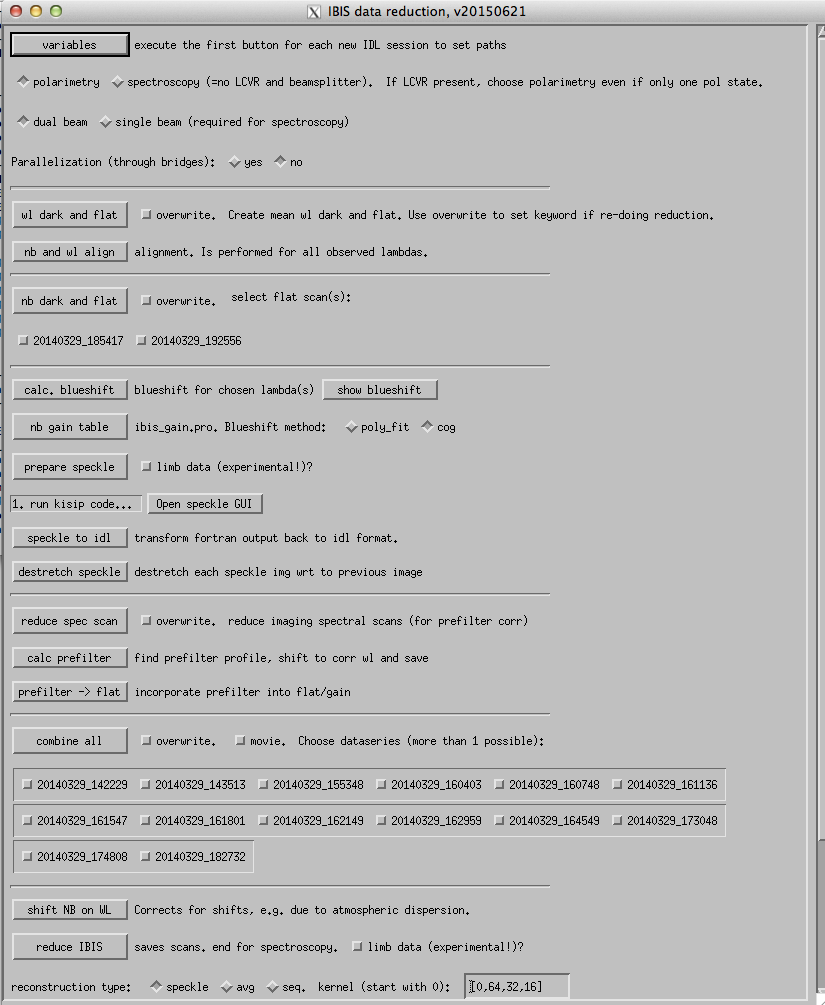
\includegraphics[width=.8\textwidth]{ibis2.png}
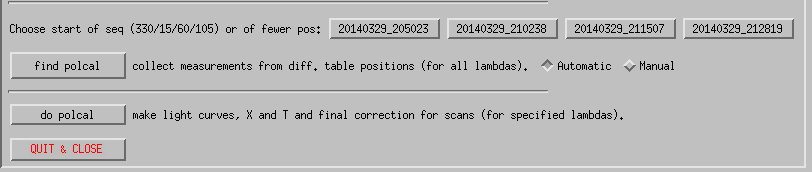
\includegraphics[width=.8\textwidth]{ibis3.png}
\caption{The IBIS GUI.\label{figgui}}
\end{figure}


\subsection{Variables}

\begin{figure}[htb]
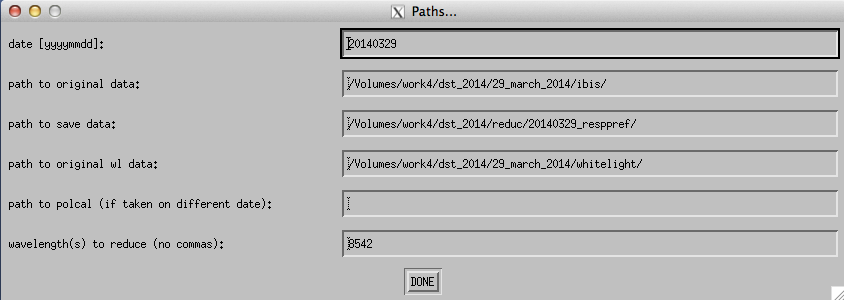
\includegraphics[width=\textwidth]{ibis1.png}
\caption{Variables for the IBIS data reduction.\label{figvar}}
\end{figure}

This is the only input required by the user (see Fig.~\ref{figvar}).\\
\textbf{date}: specify in yyyymmdd format, for example \textit{20110101} \\
\textbf{path to original data}: full path to IBIS data (narrowband) . Subdirectories will be searched.\\
\textbf{path to save data}: full path to save directory (subdirectories created automatically) \\
 The sub-structure that will be created: calibration (for cal files, flats etc.), scans (for combined WL/NB), wl (whitelight and speckle), result\_xxx (final data)\\
\textbf{path to original wl data}: full path to IBIS data (whitelight) . Subdirectories will be searched.\\
\textbf{path to tel.params}: full path to telescope parameters. Pre-2008 the telescope parameters were not in the IBIS headers and a separate camera was run to get them. This line may be left empty for newer data and will not appear in newer GUIs.\\
\textbf{path to linearity corr. curve}: The pre-2010 camera was non-linear and required a linearity correction. May be left empty for newer cameras and will not appear in newer GUIs.\\
\textbf{path to polcal}: If the polcal was taken on a different date, specify its path here in a similar format as 'path to original data'. If this line is left empty, the program assumes that the calibration was taken on the observing data and looks for the subdirectories.\\
\textbf{wavelength(s) to reduce}: for example \textit{6302 8542} or \textit{6302} (no commas)

If you get an error message, try copying ibis\_variables.txt into your current working directory.\\
Calls \textit{textbox\_lk.pro}

This step finds and creates paths and subdirectories. It restarts the GUI afterwards to initialize all measurements found (for example the polcal will go from N/A to actual timestamps).

 Calls \textit{@ibis\_reduce.pro}
  
\subsection{Observing Mode Choices}
\textbf{polarimetry / spectroscopy}: Choose polarimetry if LCVR+PBS were in the beam, even if only Stokes $I$ was measured. Spectroscopy assumes that the FOV is not restricted by the small mask. Several polarimetry programs automatically separate left and right beam. For spectroscopy, stop data reduction after reduce IBIS.

\textbf{dual beam / single beam}: If spectroscopy is chosen, single beam is required. For polarimetry, one may use dual or single beam, although the latter will be an exception and currently is not implemented (calibration would be worse and seeing polarization not correctable, but bigger FOV).

\textbf{Parallelization yes / no}: Technically not an observing mode, but mode for data reduction. If yes is selected, then destretch\_ibis will run in parallel mode using idl\_bridges. It should be significantly faster, but slightly less stable.

\subsection{WL database -> now obsolete}
Calls \textit{ibis\_wl\_db\_new.pro}

This button will no longer appear in newer version of the GUI.

For the old camera, it constructed a database of sid (seconds into the day) of white-light
images in the directory wl\_dir. This database can then be used
to find the white-light image closest in time to a given narrow-band
image. A structure for the telescope parameters is also created.

pre-2007: telescope parameters from separate camera (kodak headers)
For (early) post-2010 data the database is kept only for compatibility reasons, some variables may be required for speckle. Post-2010 data have the same filename for WL and NB, so the time difference is not used anymore to match the data.

\subsection{WL Dark and Flat}
Calls \textit{ibis\_wl\_avgdcff.pro}

This program creates a dark and a flatfield image for the whitelight camera. WL data is very simple to reduce and only requires data$_{\rm final}$ = (data$_{\rm orig}$ - dark)/flat, which is performed later.

The program prompts the user for bad scans during darks and flats. Look at the
plot and decide if any datapoints are too low/high. If you do not want
to exclude any scans, simply press enter and everything will be averaged. The WL dark image is saved in /calibration/dark\_\textit{date}.sav. The dark is subtracted from the flats and the flat image is saved in /calibration/flat\_\textit{date}.sav. Examples are shown in Fig.~\ref{figwl}.

\begin{figure}[!htb]
\begin{centering}
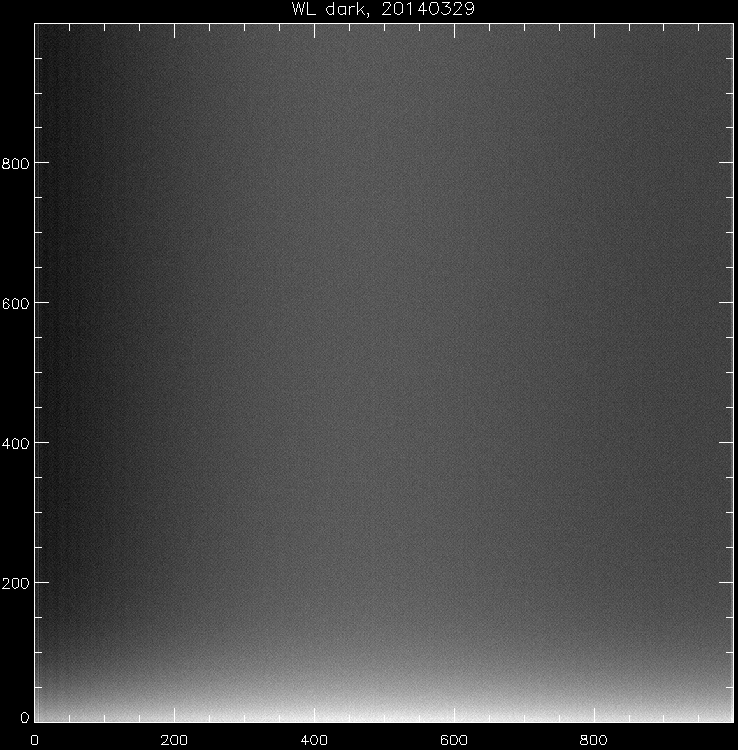
\includegraphics[width=.45\textwidth]{ibiswldark.png}
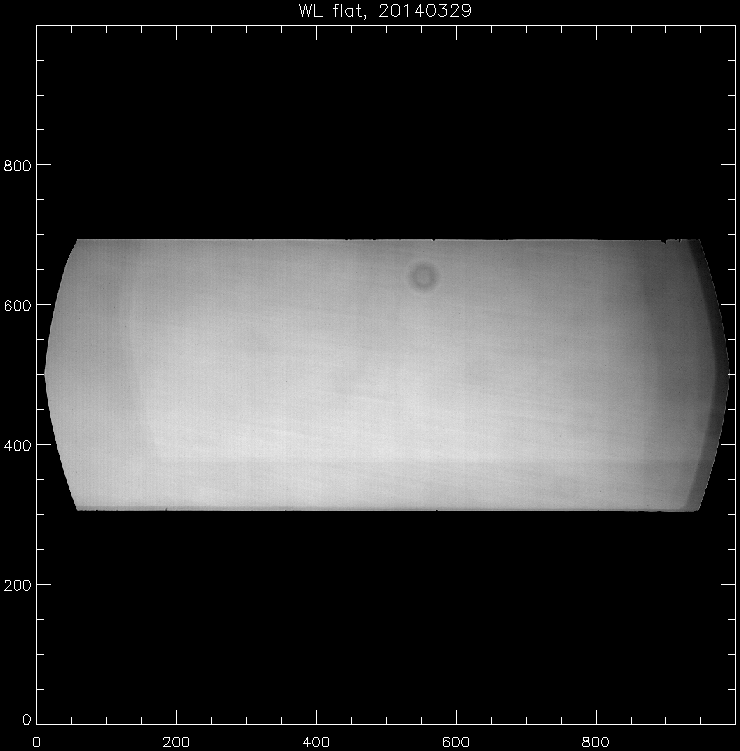
\includegraphics[width=.45\textwidth]{ibiswlflat.png}
\caption{IBIS WL dark and flat.\label{figwl}}
\end{centering}
\end{figure}


\subsection{NB and WL align}
Calls \textit{align\_ibis.pro}.


The two channels, WL and NB, (with different optical paths) need to be aligned exactly so that the destretch can be applied in future steps. This routine is completely different to NSO's version, because it does a crosscorrelation of the whole FOV, not only matching the location of 4 points.

The standard observing sequence includes dot grids and line grids. This program finds all grid files and  does not know by itself if they are dots or lines. Dots seem to work better for the alignment, but lines work too. The USAF target images are not used because they only have characters in the middle of the FOV, which does not lead to a good alignment. Look in your observing log to choose correct series (close in time to observations, because the alignment varies during the day). All observed wavelengths will be aligned, even if not specified in 'variables'.

The program prompts the user to manually rotate/mirror the images (press r) and then save the alignment (press s). This rotation parameter was different for 3 different observing runs and is therefore user-dependent. If you have trouble finding the correct orientation, look for dust on the grid.

Then, user must identify 4-5 corresponding points, first in the left,
then in the right image. This is used as first guess for
auto\_align\_images\_lk.pro. If you cannot select points (clicking has
no effect), it is probably due to a problem with X11 and cursor.pro. This happened on
my Macbook and is described here:\\
http://www.exelisvis.com/Support/HelpArticlesDetail/TabId/219/ArtMID/900/ArticleID/3947/3947.aspx
Enabling "Click-through Inactive Windows" in X11 Preferences solved my issue.

For post-2010 data, the filter and wavelength info is in the header and used to label files correctly. For older data you may need to manually write the corresponding filter and wavelength into align\_ibis.pro (variables filterindex and filterlist).


requires:\\
 ibis\_mask.pro\\
 avg.pro\\
 diffelement.pro\\
 setpts\_roi.pro (SSW)\\
 setpts\_lk.pro (modified ssw, otherwise contour plots wrong in idl 8.0)\\
 caltrans.pro\\
 auto\_align\_images\_lk.pro (modified SSW for contour plots)\\
 pq2rss.pro (SSW)\\
 anim\_lk.pro (by H. Uitenbroek, modified for modal widgets)


restrictions:\\
The new camera is chosen for observing date 2011 or later. The program
would need to be adapted for observations from aug 2010-dez 2010
 (include month in checks).

Idl 8.0 seems to have a different
contour routine making the plots look strangely compressed. My modified ssw routines
solve this problem.



PS: If one looks at the sequence of grid images during a scan, the grid is moving from image to image. Cannot be due to the AO or the actual glass plate. Possibly temperature variations? Therefore, the program uses the same extension in WL and NB for the crosscorrelation and only one image (no averaging, which would smear the dot pattern).

New in 2014: now all NB data will be aligned with respect to the broadband data. This has the advantage that final NB data should not require any cross-alignment (though a shift may be introduced by the destretch).

Updated in 2017 for single/dual beam. The offset of L/R beam is set to 0 in the single-beam case. The first guess looks bad for single beam (again issue with contour routine?), but the alignment seems to work.

\subsection{NB Dark and Flat}
Calls \textit{ibis\_dark\_avg\_nb.pro} (new cam). One dark array per filter is created.

Calls \textit{ibis\_flat\_avg\_nb.pro} (new cam).

This routine creates the dark and flatfield images for the narrowband data. The dark is one image per wavelength (even though it probably does not depend on wavelength). 

The flat scans need to be selected from the suggested timestamps in the GUI. Use at least 30 scans. For the old cam, one needs to specify nmax if the scans were aborted. Otherwise the program crashes reading a shorter-than-expected logfile. This option is not shown and unnecessary for the new cam because files are searched with file\_search() and aborted series do not matter. The output is a flat array where equal wavelengths and stokes states are averaged into one image.

\subsection{Calc.~Blueshift}
Calls \textit{ibis\_blueshift.pro}.

This routine calculates the blueshift of the instrumental profile (redshift of the spectral lines) induced by the collimated mount of the Fabry Perot. It uses flatfield data.

Procedure: load NB flat and dark, order flat by ascending wavelength, average all images of same wavelength and polarization state. Updated flat is saved, old flat is now called .backup. The user manually selects a wavelength range to use for blueshift calculation (once per prefilter) to avoid double lines as in 6301/6302. Calls \textit{ibis\_blueshift\_map.pro} to get the actual blueshift.

Blueshift calculation:\\
- Wavelength scale is interpolated to 10 m\AA\ grid because observations usually are not equidistant in wavelength. Data are interpolated (quadratic interpolation) on this scale. Left and right beam are treated separately.\\
 - Find line center for each pixel (COG, poly\_fit)\\
-  surface fit for this map with degree 2, (average all fits for each pol. state -> one map per filter)\\
- The blueshift in m\AA\ is saved with negative numbers near the center of the FOV and positive numbers towards the edges. 

\begin{figure}[!htb]
\begin{centering}
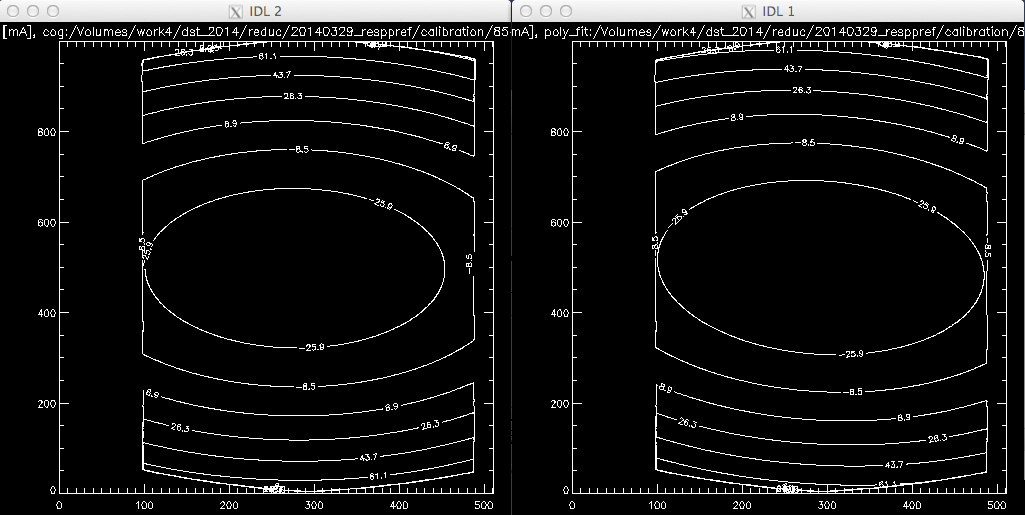
\includegraphics[width=.9\textwidth]{ibisblueshift.png}
\caption{IBIS blueshift example for 8542 \AA. Left: COG calculation, right: poly\_fit. The same contour levels are shown in both images.\label{figbs}}
\end{centering}
\end{figure}

 \begin{figure}[!htb]
\begin{centering}
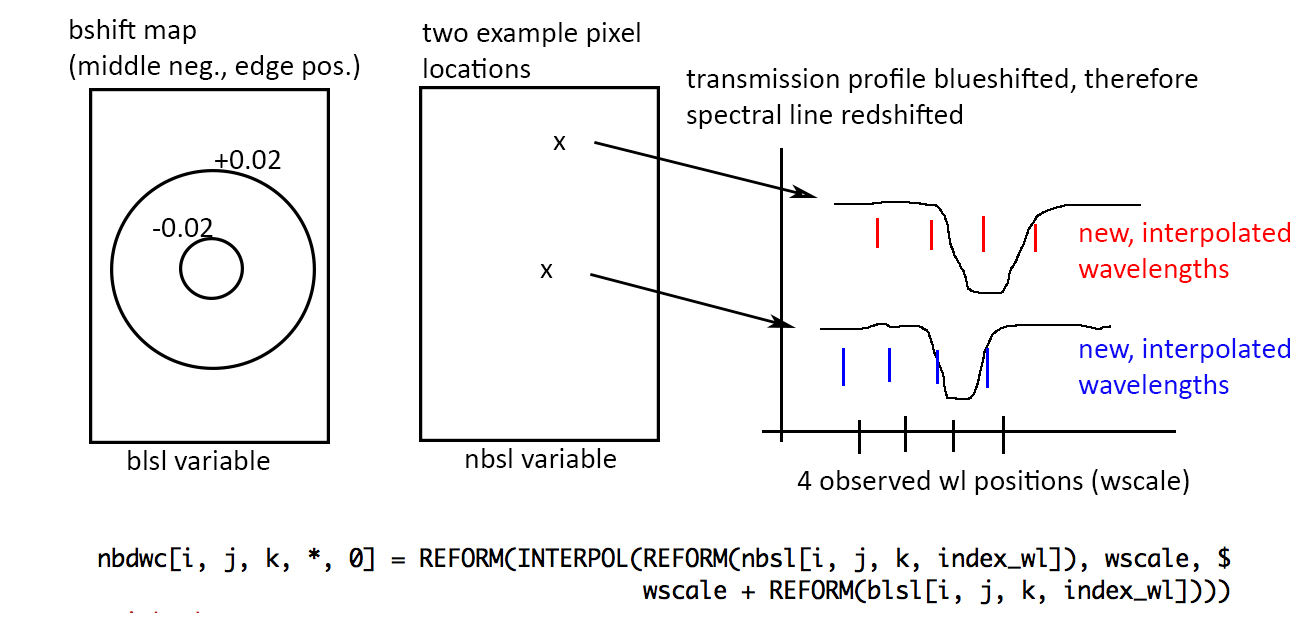
\includegraphics[width=.9\textwidth]{ibis_blueshift_scheme.jpg}
\caption{Simplified scheme of IBIS blueshift correction. Left: Negative numbers are in the middle of the FOV, positive shifts near the edges. Middle/right: Locations and spectral line of two example pixels. The spectrum from near the edge is redshifted (!), which is due to the blueshift of the passband. All profiles are interpolated onto a new wavelength scale (red and blue lines), which is then a common scale for all pixels.\label{figbs2}}
\end{centering}
\end{figure}


The routine loops through wavelengths chosen in 'variables'. If a blueshift for a certain wavelength already exists, the program asks if it should be overwritten.

The maps can be viewed with the button on the right that calls \textit{view\_blueshift.pro} and an example is shown in Fig.~\ref{figbs}. Figure~\ref{figbs2} shows the graphical principle of the correction.


\subsection{NB Gain Table}
This routine calculates the gain table of the narrowband data. The NB gain needs to be constructed without influence from the blueshift, which is why the blueshift needs to be calculated earlier and removed in this routine. Otherwise the gain would show concentric rings in the FOV.

Choose in the GUI which blueshift file should be used: poly\_fit (=polynomial fit) or COG (center-of-gravity). COG seems to be more stable if the camera has fringes or if the line is as broad as 6563.

Calls \textit{ibis\_gain.pro}

Procedure:\\
 - interpolate the wavelength of each pixel in flat to a common 10 m\AA\ scale -> average FOV -> get one ``master flat'' profile\\
 - create a shifted map of this average profile with the shift according to the values from COG or POLY\\
-  calculate the intensity difference between left and right beam (cfactor)\\
-  To calculate the flat without spectral lines: measured flats / (shifted ``master profile'' map)


Update June 2015: The ``master'' profile is now constructed from a 100x100 px box centered in the mask (with no error catching if this box ends up where it shouldn't, since I want the program to crash then to find the error). This ensures that variations due to the blueshift of the prefilter transmission profile are taken care of automatically, because averaging over a larger region would lead to a broadened ``master'' profile.

\subsection{Prepare Speckle}
\label{prepspeckle}
Calls \textit{ibis\_reduce\_speckle.pro} or \textit{ibis\_reduce\_speckle\_ncam.pro} 

For the post-2010 camera, there currently is one speckle file per IBIS reduced file (i.e. if one fits contains 6302 and 8542, then there will be 2 speckle files - one for the WL taken simultaneously to each wavelength). The burst size is given by the number of extensions with the same prefilter. I.e.~ if one observes 20 wavelengths of 6302 (polarimetry) and 15 wavelength of 6563 (Stokes $I$ only), then the burst size for 6302 will be 20*6 and for 6563 only 15, which is too low for a good speckle. The ideal size is around 70 files / burst.

So far, there is no way to save multiple files of same timestamp or to combine different files for a larger burst size. Also the program will probably crash if anybody used the repeat option (R>1) while observing. This would be a major change, because it makes finding the correct reconstruction for an observation much harder.

The program creates all ibis\_wl\_* files, which are in binary little-endian format. They only contain the actual image, whose size will be smaller than the 1000x1000 chip size.

Creates \texttt{speckle\_dims.txt} and \texttt{speckle\_sid.sav} which contains speckle\_db.

The parameters for speckle are saved in speckle\_dims.txt. Look for the pixel size of the image, and the images per burst for each wavelength in the lower part of that file to be able to properly set the parameters in the KISIP code. speckle\_db is necessary for destretch speckle (Sect.~\ref{destrsp}).

\textit{to do: create input files for speckle automatically.}

Speckle needs to be run manually! If you do not do speckle, you can omit sections \ref{prepspeckle} - \ref{destrsp} and continue with combine and choose 'avg' or 'seq' for alignment later.

\subsection{Open speckle GUI}
\label{sgui}

There is a speckle GUI written by Fred, which uses GraphApp commands. I could not get it to compile on Mac OSX.
This GUI does exactly the same (creating the 3 files init\_file.dat,
init\_method.dat and init\_props.dat), but has additional options to
display the reconstructed data. 

One may also launch the speckle reconstruction from the last tab in
the program. Be sure to set the image size, the number of images (from
speckle\_dims.txt) and
the number of speckle files in the appropriate fields. 

\textit{To do: read speckle\_dims.txt and make speckle automatic}


\subsection{Speckle to IDL}
\label{stoi}
Calls \textit{ibis\_prepare\_speckle.pro}.

Converts speckle binary files (*.final) to IDL save files (*.sav). Their original size (usually 1000x1000) is restored.

\subsection{Destretch Speckle}
\label{destrsp}

Calls \textit{ibis\_detr\_speckle.pro} (own program).

This program destretches all speckle images, meaning that the solar evolution is better visible in the final data. First, it finds all *.sav images, then it orders them by time using info from speckle\_db. When the timestamp changes, the program checks by cross-correlation if the same target was still observed and if yes, the destretch continues. Otherwise it starts a new destretch round with the first image of the series being the reference. The reference image keeps changing throughout the series to take solar evolution into account. The program overwrites all *.sav files to save space. The original *.sav files can be recreated fast with `speckle to idl'.

The program only works with post-2010 cam data. The older data that I have already looked good without it.

A hard-wired kernel of  ds\_kernel = [0,64,32] is used. It is probably not perfect, especially for data with bad seeing, but adding another level would be much slower.


\subsection{Reduce Spec Scan}
Calls \textit{read\_imagingspecscan.pro}

Finds all imaging spectral scans, asks which one to use if multiple are found. Dark-corrects (watch the exposure times!) and blueshifts the spectral scan data to be able to get a single average profile of the spectrum convolved with the prefilter transmission.

The average profile and a relative wavelength scale are saved in calibration/ imgspecscan\{wl\}.sav

\textbf{Warning}: The program will crash if the images are not 1000x1000 or larger. One needs to change xl, xr, y1 and y2 in the routine to redefine the area to be averaged for other image sizes.

\subsection{Calc Prefilter}
Calls \textit{ibis\_corr\_prefilter.pro}

The goal is to find the shift of the prefilter profile, which was measured by the PMT and thus has a different optical path and a relative wavelength offset to other data. The steps are:\\
1) broaden atlas by IBIS FWHM and shift atlas to correct minimum (strangely, my copy of the FTS atlas has a 40 m\AA\ shift of the 8542.1 line for example)\\
2) Cross-correlate flat to atlas to find the wavelength-offset of the data\\
3) compare info\_flat\_short.grid and info\_flat\_short.wave (relative/absolute wavelength) to find offset to absolute wavelength (wscale)\\
4) shift prefilter relative to spectral scan for best match (crosscorrelation) with atlas\\
5) save prefilter wavelength scale (new) and prefilter transmission

Warning: So far, this routine is only useful for 6302, 6563, 8542, 6173, 5434. For other lines, the program would require a prefilter file (done by Kevin and available in directory, but not ready to use) and some modifications (hardwired) such as the wavelength of the theoretical line center in air, an optional wavelength shift of the FTS atlas, and setting the region for cross-correlation manually (to exclude telluric lines for example).

Note that the fringes of the prefilter are not taken into account currently. It is therefore normal to see a sinusoidal continuum with an amplitude variation of ~2\% in the final data. This would require implementing a crosscorrelation with the fringe pattern derived by Kevin.

\subsection{Prefilter -> flat}
Calls \textit{flat\_prefilter.pro}

For each lambda, this program finds the gain file, the prefilter file and overwrites (!) the previous gain by
$$gain = gain / ip\_pref $$ where ip\_pref is the prefilter profile interpolated at the observed wavelengths.
This process ensures that the prefilter correction is applied to the data automatically when the gain table is applied. It has no influence on X-matrices or response matrices, because they are normalized to their first element, meaning that the intensity stays constant.

An info variable is added to the corrected gain files to avoid future prefilter corrections.



\subsection{Combine All}
Calls \textit{ibis\_combine\_ncam.pro} 
Calls \textit{assign\_speckle2nb\_ncam.pro}.

For the selected timestamps, this creates idl save files of the scans
in the \textit{temporary} directory. Darks and flatfields are also
applied. This is done for ALL observed wavelengths, independent of your selection of variables. In case this step crashes in the middle, you will need to set 'overwrite' to redo it.

A speckle database is created so that reduce IBIS can figure out which
speckle file (those only have numbers 000, 001, 002, ... instead of
actual timestamps) corresponds to the current data.

Note that if the gain was not corrected for the prefilter, this step will still work. But it is best to create gain files and prefilter profiles for all observed wavelengths (to be set in variables), before doing this step.


\subsection{shift NB on WL}
Calls \textit{ibis\_shiftatmosdisp.pro} 

On 20140306 it was noticed that the alignment of the target images only is good for rotation and scaling. In the science data, there is an extra shift between NB and WL data, probably due to atmospheric dispersion. It can reach up to 15 pixels in the mornings and evenings according to a calculation by Kevin. Shifts of 11 px were easily found. Therefore, one needs to crosscorrelate the NB data directly to the BB data, which needs to be done in the photospheric line wing to have similar features. 

This routine will restore the sav files created by 'combine' and check if the variable atmshift already exists in the file. If yes, then the correction was already done, but otherwise the user will have to interactively determine if the crosscorrelation is sufficiently good. So far, this is done for every single file manually, because we are not sure yet how much of a drift to expect with time.

Note: There are two different opinions whether this step is needed. If the turbulence occurs close to the telescope, then this step may need to be omitted because the turbulence should depend on the pixel location on the camera and not the solar region. In this case, one should do the destretch applying the same vectors to the same pixels in 8542/6302 (independent of the solar features there) and find the shift due to dispersion between the wavelengths after the destretch. However, because the seeing depends on wavelength anyway, both options may not be great and the shifts may need to be scaled down for longer wavelengths. I have never compared any of these options.


\subsection{reduce IBIS}
Calls \textit{ibis\_calibrate.pro}

This program does the actual destretch, blueshift correction, and
alignment of the files in the selected directories. The results are
saved in the timestamp-subdirectories from where the reduction is performed.

This part uses the timestamps that are checked above in the GUI and the 'cog' or 'poly' method for the blueshift. 'cog' works better for 8542 and 6563, 'poly' may work better for 6302. Therefore, it is recommended to run this step twice with different entries in 'variables' and selecting the appropriate blueshift method for the selected wavelength.

April 2017: Dual beam polarimetry and single beam spectroscopy are tested and should work. Single beam polarimetry does not work (not tested, not adapted) and currently has 'stops' in my places. Single beam spectroscopy is not parallelized (bridges and no\_bridges routines are identical).

\subsection{Find Polcal}
Calls \textit{collect\_ibis\_polcal.pro}

Creates subdirectories polcal\_xx that contain one file per wavelength per calibration sequence (000-027). These files contain nb\_data = [x,y,stokes*wavelengths]. The number of wavelengths here is low (5-6) since the polcal is assumed to be constant over the spectral line and it can be run much faster without too many wavelength points.

Make sure that you check the observer's log to see if any polcal was
aborted. In this case, select the correct timestamps
before you press 'find polcal'.

\subsection{Do Polcal}
\label{sec:polcal}
User first needs to select which directories to calibrate. Program then displays red boxes denoting the FOV of the left and the right beam. If those looks ok (should be most of the time), press (a), otherwise press (c) and click on lower left then upper right of L beam, then lower left or R beam.

The proper T-matrix (telescope calibration) is chosen automatically by date of observation.  The newest one is from May 2010 and the mirrors most likely have been recoated since, but no newer file is available [in July 2016].

 Calls \texttt{ibis\_get\_polcalcurvec}. This program first finds all sav files in the polcal subdirectories. Not all 4 table positions are required, even with 2 positions, the calibration is the same. First, the darks are subtracted from the polcal. Then, the data are put into the state [1. , state2/state1, state3/state1, state4/state1, state5/state1, state6/state1]. This means that 6 modulation states are hardcoded and that only the normalized Muller matrix of the instrument is determined. One assumption for the cal is that the lightlevel remains constant during the measurement of the six modulation states. Intensities at each y-pixel are kept, while one averages over x-pixels, i.e. the response matrix will be determined for each pixel along the long axis of the IBIS FOV. The telescope info and the polcal intensities are saved in  e.g. calibration/20140329\_polcal\_8542.sav.
 
Note November 2014: X is calculated for y-pixel and wavelength now, but the average of the FOV is still being used for the polcal (found no real improvement by using y-dependent X matrix).

The next routine called is  \texttt{ibis\_polcal\_xcalc\_v4}. Its goal is to derive the response matrix, i.e. the 4 $\times$ 6 matrix $X$, which transforms the observed modulated intensities $S'$ (I+Q, I-Q, I+V, I-V, I+U, I-U, however the names of the states have nothing to do with the actual polarization state) into the solar S (I, Q, U, V). 
\begin{equation}
S' = X T S
\end{equation}
 The telescope matrix $T$ is used during the fitting. The actual fitting is done with mpfitfun, which is run in parallelized mode for each wavelength point (by calling \texttt{aux\_xcalc\_v4}), otherwise it would take $>$1h for the usually 6-7 wavelength points. There are 28 free parameters: 24 matrix entries, the waveplate offset, the waveplate retardance, the waveplate dichroism and the linear polarizer extinction. One may have to install for\_split.pro to make the parallelization work. The output is saved as e.g. 01.ta.20140329.8542.X.idl for the left beam and 01.tb.20140329.6302.X.idl for the right beam. The dimensions of xmat are Array[4, 6, 903, 8], meaning 4x6 matrix for 903 y-pixels and 8 wavelength points.

The main program (IBIS GUI) then queries the user for a region of quiet Sun, later to be used for crosstalk calibration. Savefile: \texttt{qsreg.txt}. If the file already exists, the QS region is not displayed anymore.

The IBIS GUI then queries for the choice of continuum (choose left edge and right edge, ideally 2 wavelength points) and saves it in cont\_8542\_sav.

For the actual calibration of the data, \texttt{main\_ibis\_calibrate\_v2} is called. It restores the response matrices for both beams and the T-matrix and calls several subprograms: 


\begin{minipage}{0.05\textwidth}\hfill
\end{minipage}
\begin{minipage}{0.95\textwidth}
It calls \texttt{ibis\_scan\_calibrate\_xt\_v2}, which by default averages the X-matrices over y-pixels (other options include smoothing and linear fitting should be implemented) and wavelength. It then inverts the 4x6 matrix via SVD and interpolates it for each observed wavelength step (which has no effect, since the wavelengths were averaged, but this could be used for wavelength-dependent X-matrix calibrations). The telescope matrix is 4x4 and is inverted with INVERT().
The program then loops over all pixels and calculates $T^{-1} \#\# X^{-1} \#\#$ pixel, giving the normalized observed Stokes vector (I, Q, U, V). Left and right beams are then combined as
\begin{eqnarray*}
I = 0.5 * (I_L + I_R) \\
Q = 0.5 * ((Q_L / I_L) + (Q_R/I_R)) * I \\
\cdots
\end{eqnarray*}
to account for different beam intensities (beam balancing).

If the keyword region is set (by default it is), then the quiet Sun is used to correct for I$\rightarrow$Q,U,V crosstalk via \texttt{ibis\_scan\_xtalk\_i2quv}. The continuum points that the user chose are used to average to a continuum value of I,Q,U,V. For the QS region that the user selected, the fractional polarizations Q/I, U/I and V/I are calculated (in the continuum). Those are the values polfac = [polfacv, polfacq, polfacu] that are also saved later. The corrections for the crosstalk calculates e.g. V$_{new}$ = V - polfacv $\cdot$ I. Note: the residual crosstalk (V$\rightarrow$Q,U and Q,U$\rightarrow$V) is not corrected, because it led to strange results and shall be done manually if necessary.

Q and U are then rotated into the correct solar reference frame, which depends on the solar P angle and uses a calculation of which I have no clue what it does.

The calibrated data are saved as e.g. 6302\_nb027.pc.tatb.sav, pc standing for polcal and tatb for both beams. This is the final step of the pipeline.

\end{minipage}








%\subsection{do prefilter corr}
%Calls \textit{apply\_prefilter.pro}
%
%Overwrites (!) all reduced data with a new, corrected stokesout. Basically, stokesout$_{\rm new}$ = stokesout$_{\rm old}$ / (prefilter, interpolated at correct wavelengths). This is done for all polarization states. An info variable is added to the corrected files to avoid future prefilter corrections.

%This part uses the timestamps are are checked above in the GUI.



\section{Versions and changes}

v170413
\begin{itemize}
\item Adapted and tested pipeline for single-beam. Many functions were adapted. No changes to dual-beam methods, apart from finding bug in atmospheric dispersion routine (atmosdisp), which only applied shifts to L beam in the past and not R beam.
\item Aug 9, 2017: Updated manual to include a description of IBIS and the general reduction steps.
\end{itemize}


v150621: June 2015
\begin{itemize}
\item Until now, the prefilter correction was applied as a last step. This is incorrect, because it should be applied before the demodulation. Also, the spatially varying (blueshifted) prefilter transmission profile needs to be taken into account. Therefore, construct the ``flat'' profile only from a small box (100 x 100 pixels around the center of the mask), otherwise the prefilter transmission changes would be divided out. The prefilter correction is now applied to the gain, which will automatically correct the data. Note that differences to data with the old prefilter correction are minimal, especially near the center of the prefilter (where the spectral line usually is).
\item Fixed possible crash if user selected wrong corner for rigid alignment feature
\item All prefilter files are now available, but not implemented (requires changing variable names and some hard-wired parameters, such as locations of telluric lines). Currently, the prefilter correction works for 8542, 6302, 6173, 6563, 5434. Let me know if you need another filter.
\item Updated manual in March 2016 to contain some figures and examples.
\item Updated manual in July 2016 to explain polcal in detail.
\end{itemize}


v141114: November 2014
\begin{itemize}
\item Polcal was found to depend on spatial y (long axis of IBIS mask) and wavelength, especially far from line center. Now X-matrices are computed with more dimensions and less averaging. Implemented parallelization of X-computation. The spatially dependent X-matrix however did not solve the calibration issues for 6302 on 20140329. For 8542, a constant matrix has always worked. Therefore, the default is currently to still calculate and save the spatially dependent X, but then average over the FOV and only apply one X-matrix per beam (can be modified in main\_ibis\_calibrate\_v2.pro:84 by removing the /avg keyword).
\end{itemize}


v140221: January/Feb 2014
\begin{itemize}
\item Support for old camera dropped (use v5 for that).
\item Alignment done with respect to whitelight images. All wavelengths should thus be aligned.
\item speckle\_gui implemented that can run the speckle code and display reconstructed images
\item GUI is now based on pointers instead of common variables.
\item Polcal should work with fewer than 4 table positions. 2 are
  recommended, 1 is required.
\item Atmospheric refraction was discovered to be significant. Now NB data can be correlated to WL data for each scan.
\end{itemize}



v5: 2013
\begin{itemize}
\item More or less stable reduction.
\end{itemize}



v4: May 4, 2012:
\begin{itemize}
\item completely cleaned up the ibis\_v4\_lucia directory. Now it should contain all necessary routines to run the reduction.
\item substituted the old ASP cal with a new polcal written by T. Schad. The old cal required many more routines, was a lot less understandable and the resulting X matrices are the same in both versions.
\item Enabled logging. A .tex log containing  each performed step is saved in the \textit{log} subdirectory.
\item Many bug fixes, especially for the old camera, but also for the alignment procedure and the beam combination (beam balancing by T. Schad). The region for the polcal is now guessed by the program. The region for rigid alignment is now saved for each timestamp, not globally.
\item T. Schad implemented a parallelization of the destretch using IDL bridges. The default setting is off in the GUI because it might be a little unstable, but it can be enabled by checking the box.
\end{itemize}

v3: 2012:
\begin{itemize}
\item implemented prefilter correction
\end{itemize}

\subsection{ToDo and known problems}

\begin{itemize}
 \item Limb data have issues during the reduction due to gradients (alignment and speckle fails). There is a /limb keyword, but it would require some modifications and will currently stop/crash. The option assumes\\
      a) the limb is vertical in the image\\
      b) there is a sunspot located at some fixed coordinates which must be changed manually 
         (to avoid center-to-limb calculation at that point). change in: \mbox{ibis\_reduce\_speckle.pro:154} and
            ibis\_calibrate.pro:447
     limb does not work with the new camera yet!

\item single beam polarimetry may have stops in the code because it has never been tested.
\item cog blueshift seems to be better than poly\_fit for new cam (which has fringes). But for 6302 poly\_fit seems better. Currently the user has to choose manually.
\item speckle for new cam makes 1 burst per wavelength per fits file. There
  should be at least 50 images per filter (=more than ~8 $\lambda$ steps for polarimetry) for successful speckle. ToDo: Option to combine/split files for speckle
\item ibis\_flat\_avg\_nb could be faster: read s000 only (once per
  timestamp) and assume that other files (per timestamp) are the same
\item assign\_speckle2nb does not have an overwrite option. Must delete file manually if redoing speckle.
\item option R>1, i.e. repetitions of same line in fits file not supported yet.
\item autopolcal: BE CAREFUL! the labels of the buttons are suggestions, taking poldir[0,28,56,84]
    which usually will not be okay since the instrument fails at least once per calibration sequence
    and/or the series are restarted by the observers due to clouds etc.. For example, on June 12 the 
    first poldir series was also useless (which was not easily visible in the logs! the hint was that the
    log said "Iteration  \#1 of 10" instead of '\#1 of 1') so really make sure you choose the 
    correct starting directories. Currently, there is no warning if something looks strange.
\item to look at the reduced data, use view\_ibis,stokesout,lambda=wl\_obs (will be implemented in gui later)
\item the parallelization through bridges is not entirely stable. If you ever had to do Ctrl+c before `reduce IBIS' to get to the command line, the bridges will quit and need to be re-run (=do reduce IBIS again). Also, never do Ctrl+C while the bridges are running, otherwise you'll need to kill the whole terminal.
\end{itemize}


\bibliographystyle{apj}
\bibliography{journals,ref_manual}


\end{document}



